\begin{scanpage}{0047}{30}
The functions $f^1$ and $g^1$ have a finite value everywhere, except for the particular values $\phi$ and $\phi_0$ enumerated in Equation (4.04). The graphs of the functions $f^1$ and $g^1$ (Figures 8--13) drawn in polar coordinates give a visual representation of the effect of the nonuniform part of the current which is concentrated near the wedge edge. In particular, they show that this effect may be substantial for the fringing field not only in the shadow region $(\pi+\phi_0<\phi<\alpha)$, but also in the region of light $(0<\phi<\pi+\phi_0)$. The continuous lines in the figures correspond to the functions $f^1$ $(f^1<0)$. The dashed and dash-dot lines correspond to the functions $g^1$ --- the dash lines refer to the case $g^1<0$, and the dash-dot lines refer to the case $g^1>0$.
\begin{center}\begin{minipage}[t]{.48\linewidth}\vspace{0pt}\centering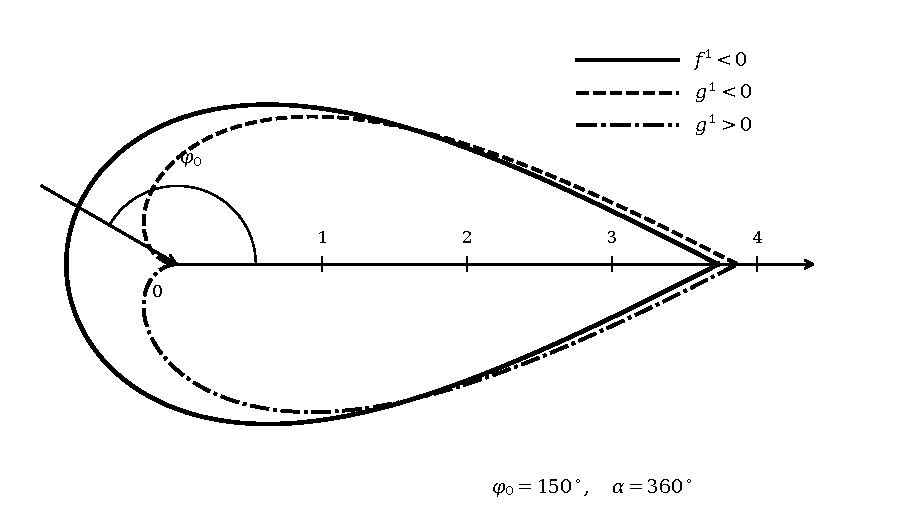
\includegraphics[width=.9\linewidth]{images/recreated/a-0047-fig8.pdf}\par Figure 8. The diagram of the field from the nonuniform part of the current excited by a plane wave on a half-plane. The function $f^1$ (or $g^1$) corresponds to the case when the electric (or magnetic) vector of the incident wave is parallel to the wedge edge.\end{minipage}\hfill\begin{minipage}[t]{.48\linewidth}\vspace{0pt}\centering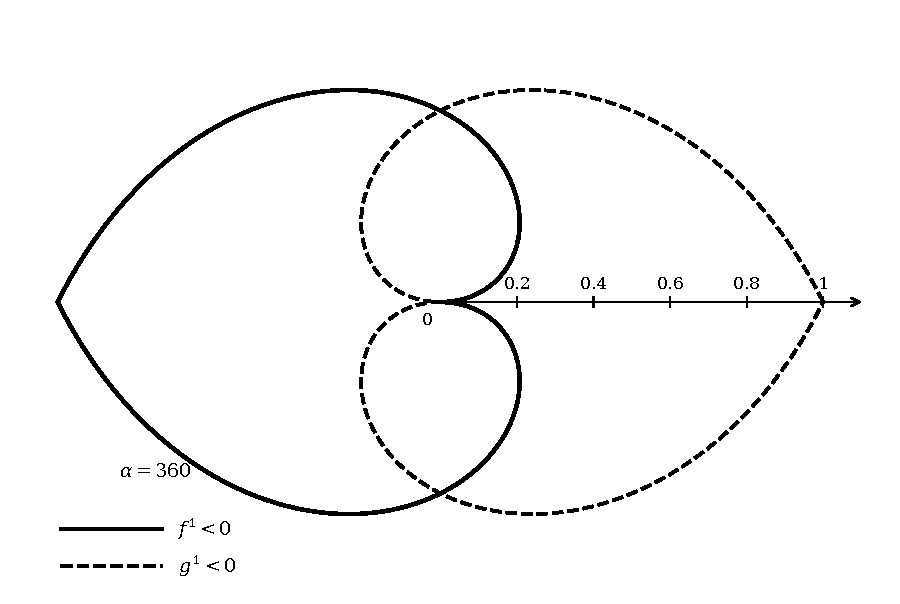
\includegraphics[width=.95\linewidth]{images/recreated/a-0047-fig9.pdf}\par Figure 9. The same as Figure 8 for the case $\phi=\phi_0$.\end{minipage}\end{center}
Let us turn our attention to the next important aspect. As is seen from \S\ 1 and 3, the nonuniform part of the current on the wedge is described by a contour integral which is generally not expressed in terms of well-known functions. But in order to calculate the field scattered by some convex, ideally conducting surface with discontinuities (edges), the indicated expression still must be integrated over the given surface. Obviously, such a path is able to lead only to very cumbersome equations. Therefore, henceforth, when calculating
\end{scanpage}
